\chapter{Interaksi Basisdata}
\section{MySQL}
%create user: create user 'arya'@'localhost' identified by '123456';
%create database: create database iris;
%grant user: grant all on 'iris.* to 'arya'@'localhost';
%flush privileges;
%create table irisdata (sepallength real(2,1), sepalwidth real(2,1), petallength real(2,1), petalwidth real(2,1), kelas varachr(15));
Modifikasi \lstlistingname~\ref{lst:bacairis} sehingga menjadi seperti \lstlistingname~\ref{lst:insertiris}. Hasil ekseksinya ditunjukkan \figurename~\ref{fig:insertmysql}.
 
\lstinputlisting[language=python, numbers=left, numberstyle=\small, caption=Membaca dataset iris dan menyimpannya di MySQL, showstringspaces=false, label=lst:insertiris]{script/insertiris.py} 

\begin{figure}
  \begin{center}
    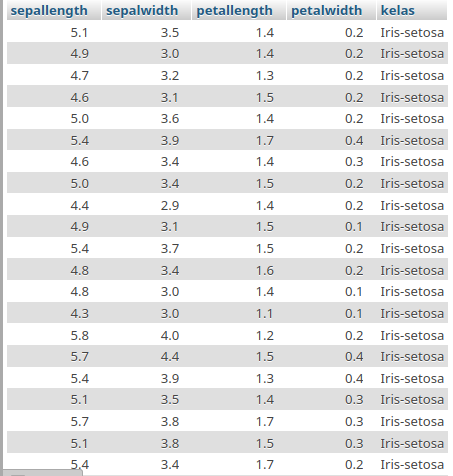
\includegraphics[scale=2.0]{pics/insertmysql.png}
    \caption{Hasil dari proses memasukkan data ke server MySQL}
    \label{fig:insertmysql}
  \end{center}
\end{figure}
\section{PostgreSQL}
Modifikasi \lstlistingname~\ref{lst:insertiris} sehingga menjadi seperti \lstlistingname~\ref{lst:insertirispg}. Hasil ekseksinya ditunjukkan \figurename~\ref{fig:insertpgsql}.

\lstinputlisting[language=python, numbers=left, numberstyle=\small, caption=Membaca dataset iris dan menyimpannya di pgSQL, showstringspaces=false, label=lst:insertirispg]{script/insertirispg.py}

\begin{figure}
  \begin{center}
    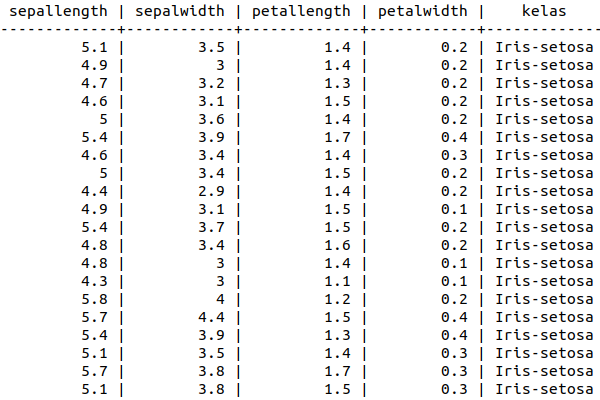
\includegraphics[scale=2.0]{pics/insertpgsql.png}
    \caption{Hasil dari proses memasukkan data ke server pgSQL}
    \label{fig:insertpgsql}
  \end{center}
\end{figure}

%https://computingforgeeks.com/installing-postgresql-database-server-on-ubuntu/
%https://linuxhint.com/postgresql_installation_guide_ubuntu_20-04/
\section{MongoDB}
